\mainentry{blinkenlights} /blink'*n-li:tz/ n.

[common] Front-panel diagnostic lights on a computer, esp. a
\citeentry{dinosaur}. Now that dinosaurs are rare, this term usually refers to
status lights on a modem, network hub, or the like.

This term derives from the last word of the famous blackletter-Gothic sign in
mangled pseudo-German that once graced about half the computer rooms in the
English-speaking world. One version ran in its entirety as follows:

\begin{quotation}
    \begin{center}
        ACHTUNG! ALLES LOOKENSPEEPERS!
    \end{center}

    Das computermachine ist nicht fuer gefingerpoken und mittengrabben. Ist easy
    schnappen der springenwerk, blowenfusen und poppencorken mit spitzensparken.
    Ist nicht fuer gewerken bei das dumpkopfen. Das rubbernecken sichtseeren
    keepen das cotten-pickenen hans in das pockets muss; relaxen und watchen das
    blinkenlichten.
\end{quotation}

This silliness dates back at least as far as 1959 at Stanford University and had
already gone international by the early 1960s, when it was reported at London
University's ATLAS computing site. There are several variants of it in
circulation, some of which actually do end with the word `blinkenlights'.

In an amusing example of turnabout-is-fair-play, German hackers have deveoped
their own versions of the blinkenlights poster in fractured English, one of
which is reproduced here:

\begin{quotation}
    \begin{center}
        ATTENTION
    \end{center}

    This room is fullfilled mit special electronische equippment. Fingergrabbing
    and pressing the cnoeppkes from the computers is allowed for die experts
    only! So all the ``lefthanders'' stay away and do not disturben the
    brainstorming von here working intelligencies. Otherwise you will be out
    thrown and kicked anderswhere! Also: please keep still and only watchen
    astaunished the blinkenlights.
\end{quotation}

See also \citeentry{geef}.

Old-time hackers sometimes get nostalgic for blinkenlights because they were so
much more fun to look at than a blank panel. Sadly, very few computers still
have them (the three LEDs on a PC keyboard certainly don't count). The obvious
reasons (cost of wiring, cost of front-panel cutouts, almost nobody needs or
wants to interpret machine-register states on the fly anymore) are only part of
the story. Another part of it is that radio-frequency leakage from the lamp
wiring was beginning to be a problem as far back as transistor machines. But the
most fundamental fact is that there are very few signals slow enough to blink an
LED these days! With slow CPUs, you could watch the bus register or instruction
counter tick, but at 33/66/150MHz it's all a blur.

Finally, a version updated for the Internet has been seen on
news.admin.net-abuse.email:

\begin{quotation}
    \begin{center}
        ACHTUNG! ALLES LOOKENSPEEPERS!
    \end{center}

    Das Internet is nicht fuer gefingerclicken und giffengrabben. Ist easy
    droppenpacket der routers und overloaden der backbone mit der spammen und
    der me-tooen. Ist nicht fuer gewerken bei das dumpkopfen. Das mausklicken
    sichtseeren keepen das bandwit-spewin hans in das pockets muss; relaxen und
    watchen das cursorblinken.
\end{quotation}

This newest version partly reflects reports that the word `blinkenlights' is (in
1999) undergoing something of a revival in usage, but applied to networking
equipment. The transmit and receive lights on routers, activity lights on
switches and hubs, and other networking equipment often blink in visually
pleasing and seemingly coordinated ways. Although this is different in some ways
from register readings, a tall stack of Cisco equipment or a 19-inch rack of
ISDN terminals can provoke a similar feeling of hypnotic awe, especially in a
darkened network operations center or server room.

\end{multicols}

\begin{figure}[h]
    \caption{\url{http://www.blinkenlights.nl/images/blinkenlights-big.jpeg}}
    \begin{new}
        \begin{center}
            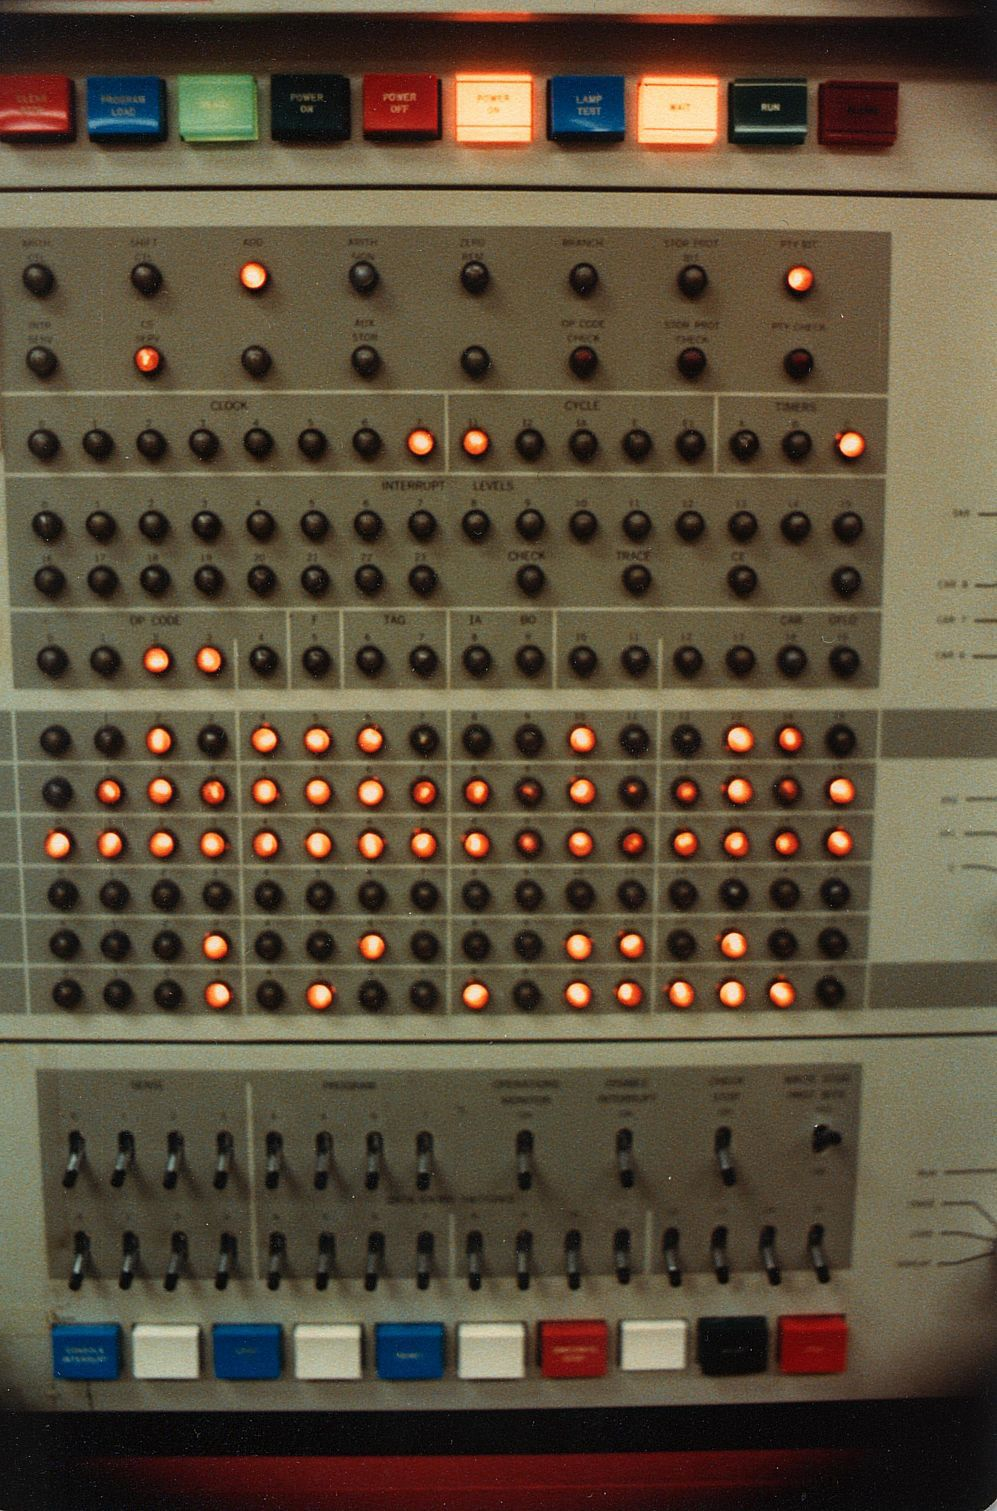
\includegraphics[width=0.5\textwidth]{img/blinkenlights-big.jpeg}
        \end{center}
    \end{new}
\end{figure}

\begin{multicols}{2}

